\chapter{Cibles de fonctionnement}

\section{Les attentes client}

Nous avons été contacté par la société SPIE Sud-Est afin d'améliorer certains points dans le processus de gestion des contrats de maintenance. Il s'agit de proposer des solutions pour :

\begin{itemize}
    \item le développement de procédures métier et de supports d'exploitation par les entités de maintenance et service
    \item la standardisation des procédures métier et de supports d'exploitation pour les entités exerçant le même métier sur le même secteur d'activité client
    \item l'analyse des risques propres à chaque métier sur le même secteur d'activité client
    \item l'amélioration de la définition des limites des interfaces avec les autres processus
    \item la mise en place d'un Info centre sur l'intranet
\end{itemize}

Les chapitres précédents --- analyse de l'existant et benchmarking --- permettent d'identifier les axes sur lesquels le système d'information de SPIE ne suit pas les bonnes pratiques, et où des améliorations sont à prévoir.

    Nous allons donc citer dans ce document certains thèmes d'amélioration possibles au travers des axes suivants~:

    \begin{enumerate}
        \item Réorganisation de la logique des processus existants~;
        \item Réorganisation des acteurs des processus métiers de SPIE pour suivre les ``best-practices'' dégagées~;
        \item Réorganisation des acteurs~;
        \item Réorganisation de l'architecture applicative~;
    \end{enumerate}

\section{Réorganisation des processus}

\subsection{Processus Retour d'expérience}

Un premier problème que nous avions identifié dans les processus actuels de SPIE-Sud-Est, est qu'il n'existe à l'heure actuel, aucun processus dédié aux retours que soit du client, ou des
differents intervenants sur le contrat. Pour cela, nous ajoutons donc trois nouveau processus au sous-processus \textit{Solde de l'affaire et du contrat}~:

\begin{description}
    \item[Retour d'expérience client] afin que les clients puissent s'exprimer sur leur expérience avec SPIE~;
    \item[Réunion retour d'expérience interne] afin que les différents intervenants sur le contrat puissent communiquer les bons et les mauvais points concernant le déroulement du contrat de manière interne~;
    \item[Bilan du contrat] afin de prendre en compte l'ensemble des retours récoltés lors des \textit{Retour d'expérience client} et de la \textit{Réunion retour d'expérience interne}.
\end{description}

\begin{figure}[h!]
	\centering
	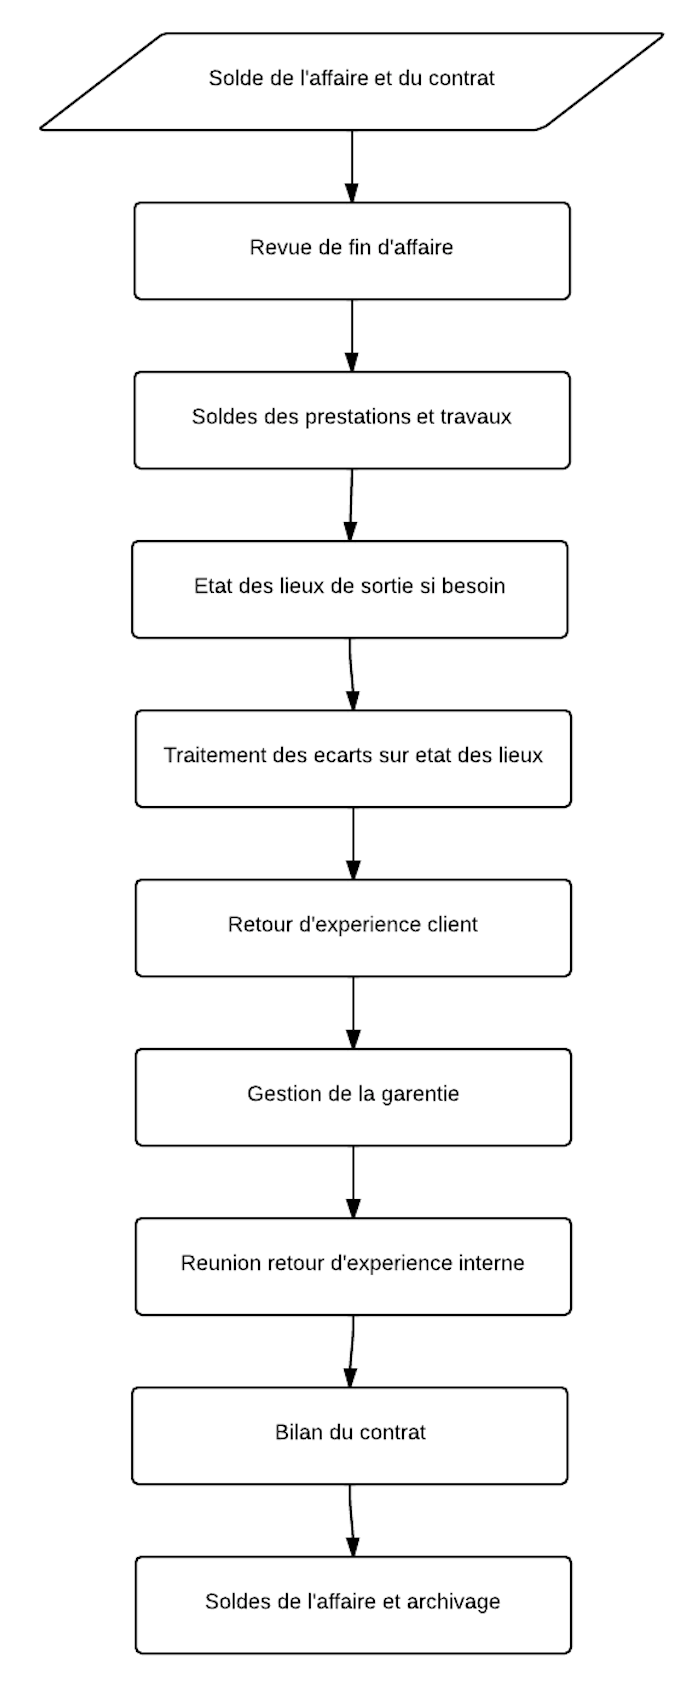
\includegraphics[width=0.45\linewidth]{images/processus_retour_experience.png}
	\caption{Sous-processus Solde de l'affaire et du contrat}
	\label{fig:processusRetourExperience}
\end{figure}


\subsection{Revue des processus}

Le second manquement que nous avions identifié dans les processus actuels de SPIE-Sud-Est, est qu'il n'y a aucun processus permettant une visibilité sur l'ensemble des processus en cours ou terminés.
C'est pourquoi nous proposons de créer un nouveau processus indépendant et parallèle aux autres, comportant deux sous-processus~:

\begin{description}
    \item[Revues des processus soldés] uniquement dédié aux processus soldés depuis la dernière revue, et qui permet de centraliser les retours sur les processus \textit{Bilan du contrat}~;
    \item[Revues des processus en cours] quant à lui est dédié aux processus en cours, afin de leur affecter les ressources matérielles et humaines nécessaires.
\end{description}

\begin{figure}[h!]
	\centering
	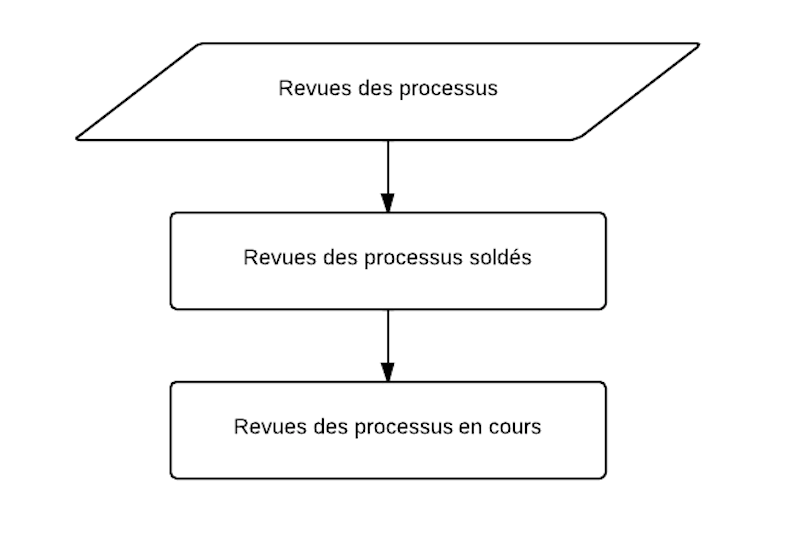
\includegraphics[width=0.45\linewidth]{images/processus_revues.png}
	\caption{Nouveau processus de revues}
	\label{fig:processusRevue}
\end{figure}

\begin{figure}[h!]
	\centering
	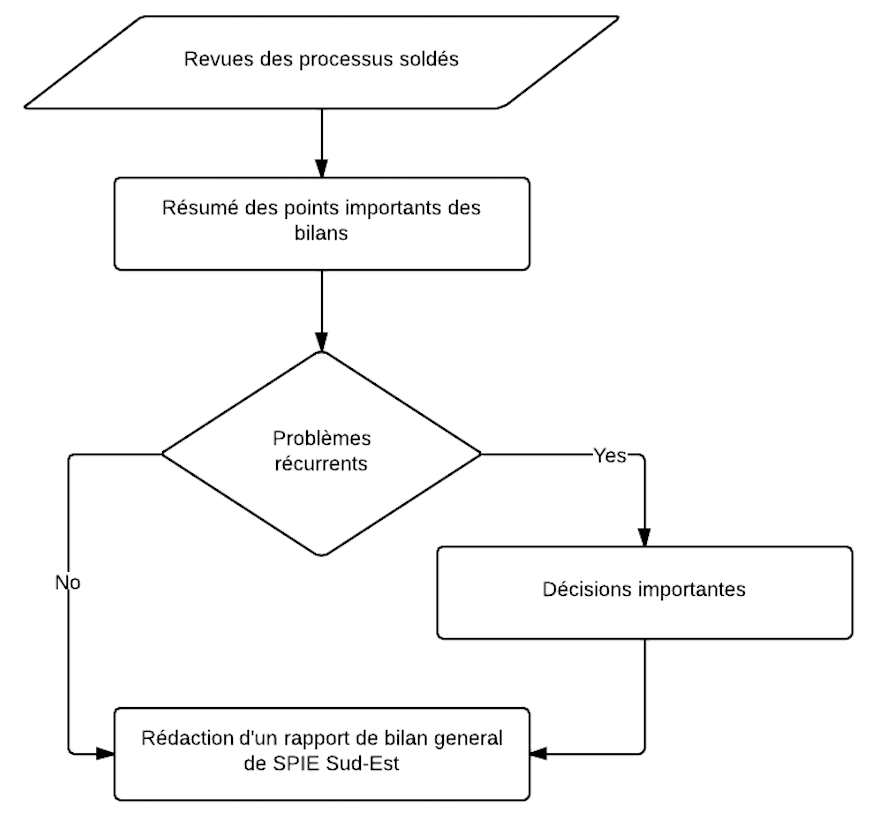
\includegraphics[width=0.45\linewidth]{images/processus_revues_solde.png}
	\caption{Nouveau processus de revues sold\'e}
	\label{fig:processusRevueSolde}
\end{figure}

\begin{figure}[h!]
	\centering
	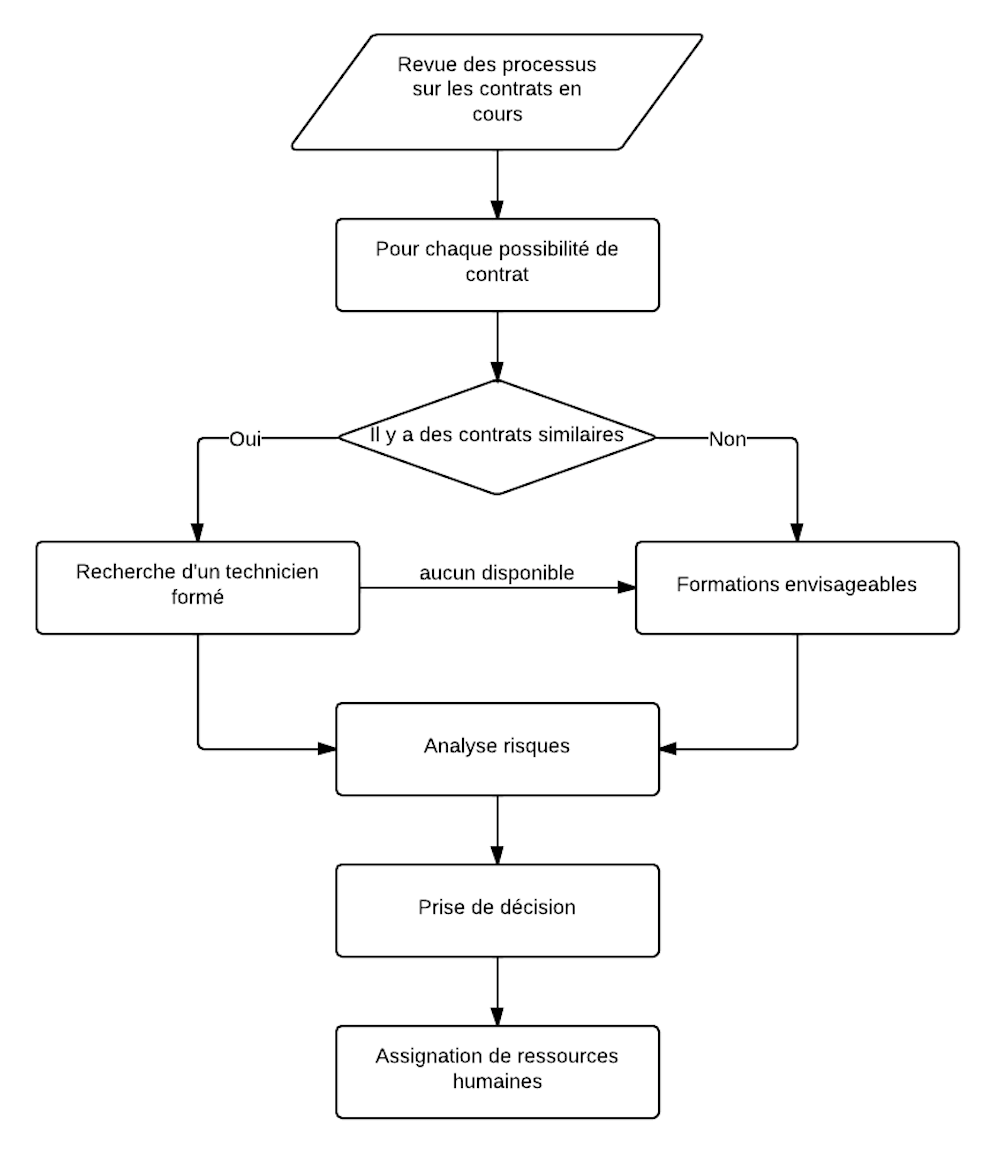
\includegraphics[width=0.45\linewidth]{images/processus_revues_actuels.png}
	\caption{Nouveau processus de revues en cours}
	\label{fig:processusRevueCours}
\end{figure}


\section{Réorganisation des acteurs}

\subsection{Diagramme des cas d'utilisation}

La figure \vref{fig:useCase} présente le diagramme de cas d'utilisation représentant les modifications apportées à l'organisation des acteurs intervenant dans le processus de maintenance.

\begin{figure}[h!]
	\centering
	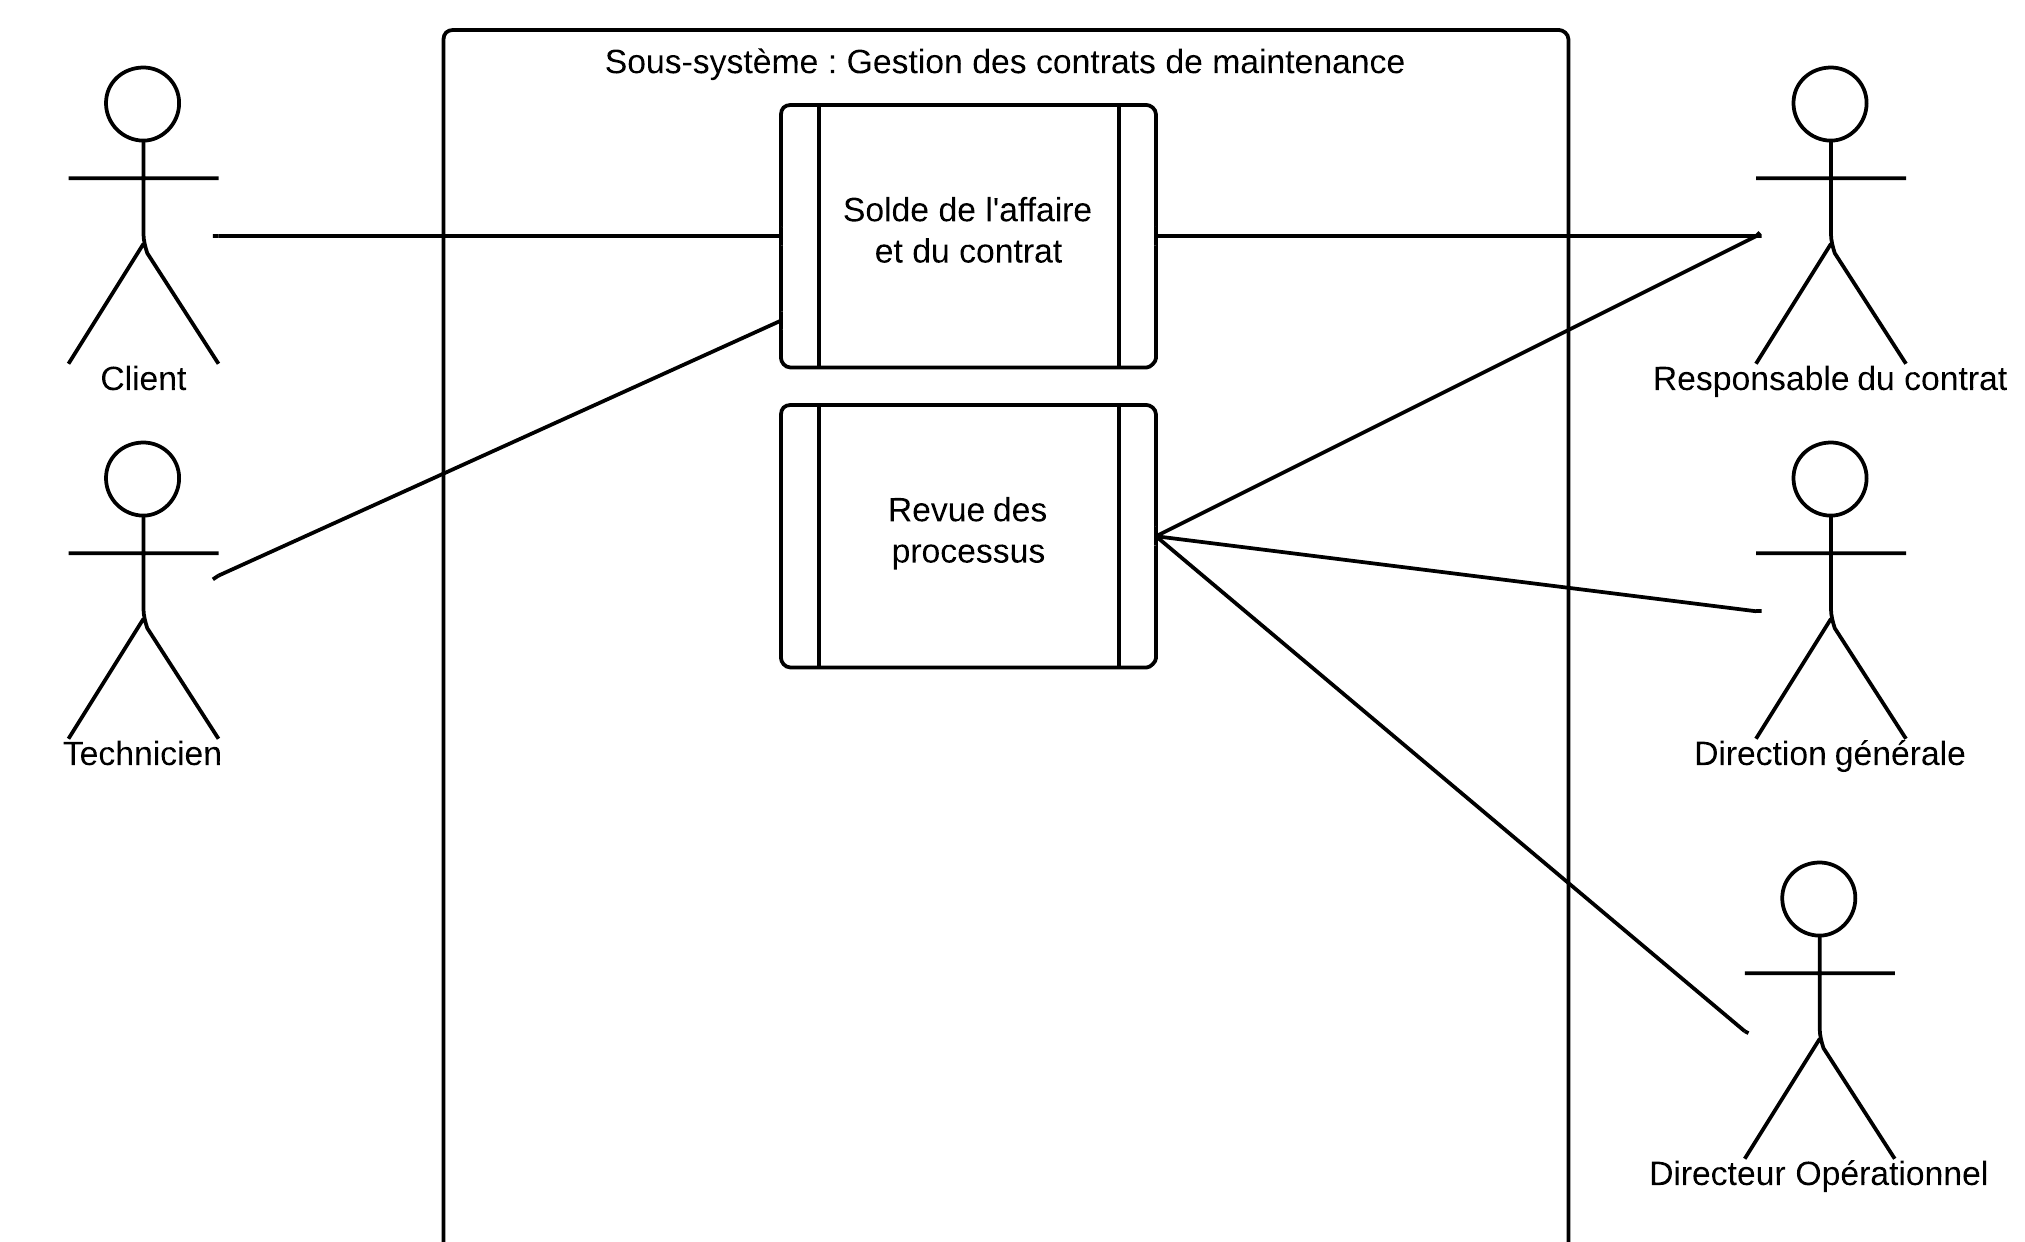
\includegraphics[width=1\linewidth]{images/useCase.png}
	\caption{Modifications apportées aux processus et acteurs}
	\label{fig:useCase}
\end{figure}

\pagebreak
\subsection{Modèle des objets métiers}

La figure \vref{fig:objets_metiers} présente les objets métiers intervenants dans les processus de gestion des contrats de maintenance.

\begin{figure}[h!]
	\centering
	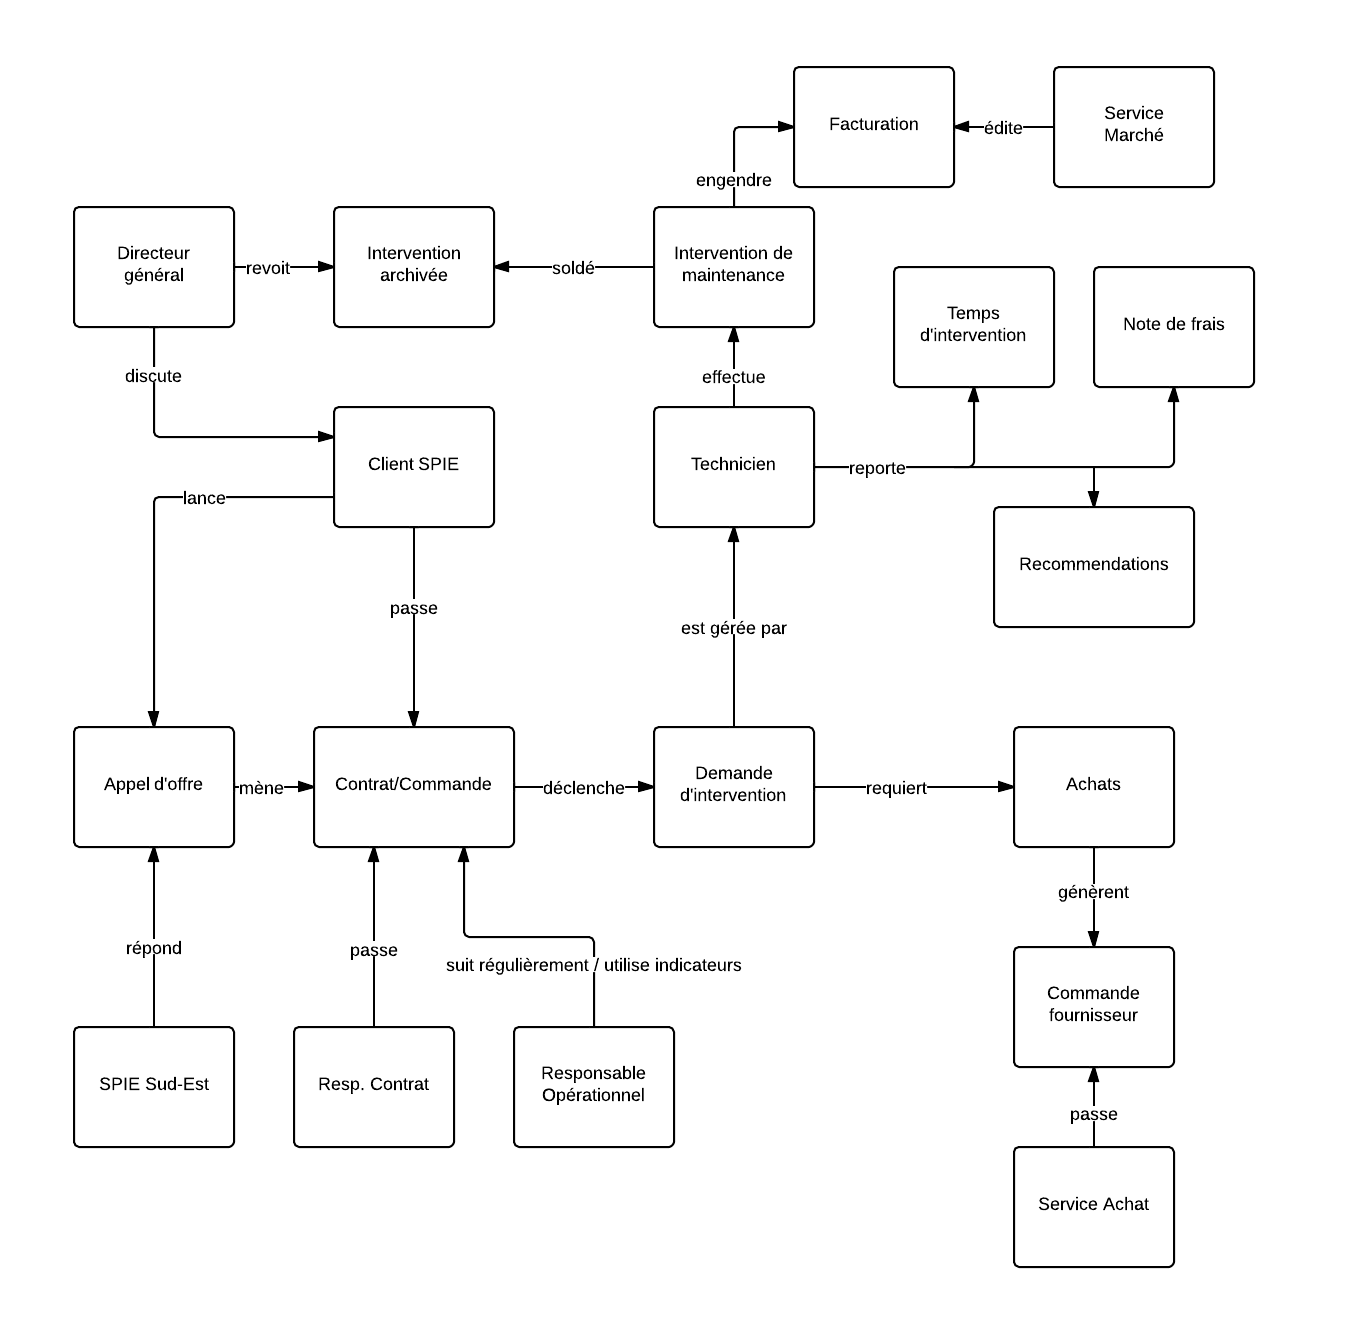
\includegraphics[width=1\linewidth]{images/modele_objet_metier.png}
	\caption{Modèles des objets métiers}
	\label{fig:objets_metiers}
\end{figure}


\pagebreak
\section{Réorganisation de l'architecture applicative}

Nous avons retravaillé l'architecture applicative afin de prendre en compte les nouvelles technologies suivantes~:

    \begin{itemize}
        \item un CRM (Customer Relationship Management)
        \item une application mobile
        \item un moteur de recommendations
    \end{itemize}

Ces nouvelles technologies sont détaillées pour précisement dans la section \vref{progres_tech}.

La figure \vref{fig:nouvelleArchitectureApplicative} présente la nouvelle architecture applicative proposée.

\begin{figure}[h!]
	\centering
	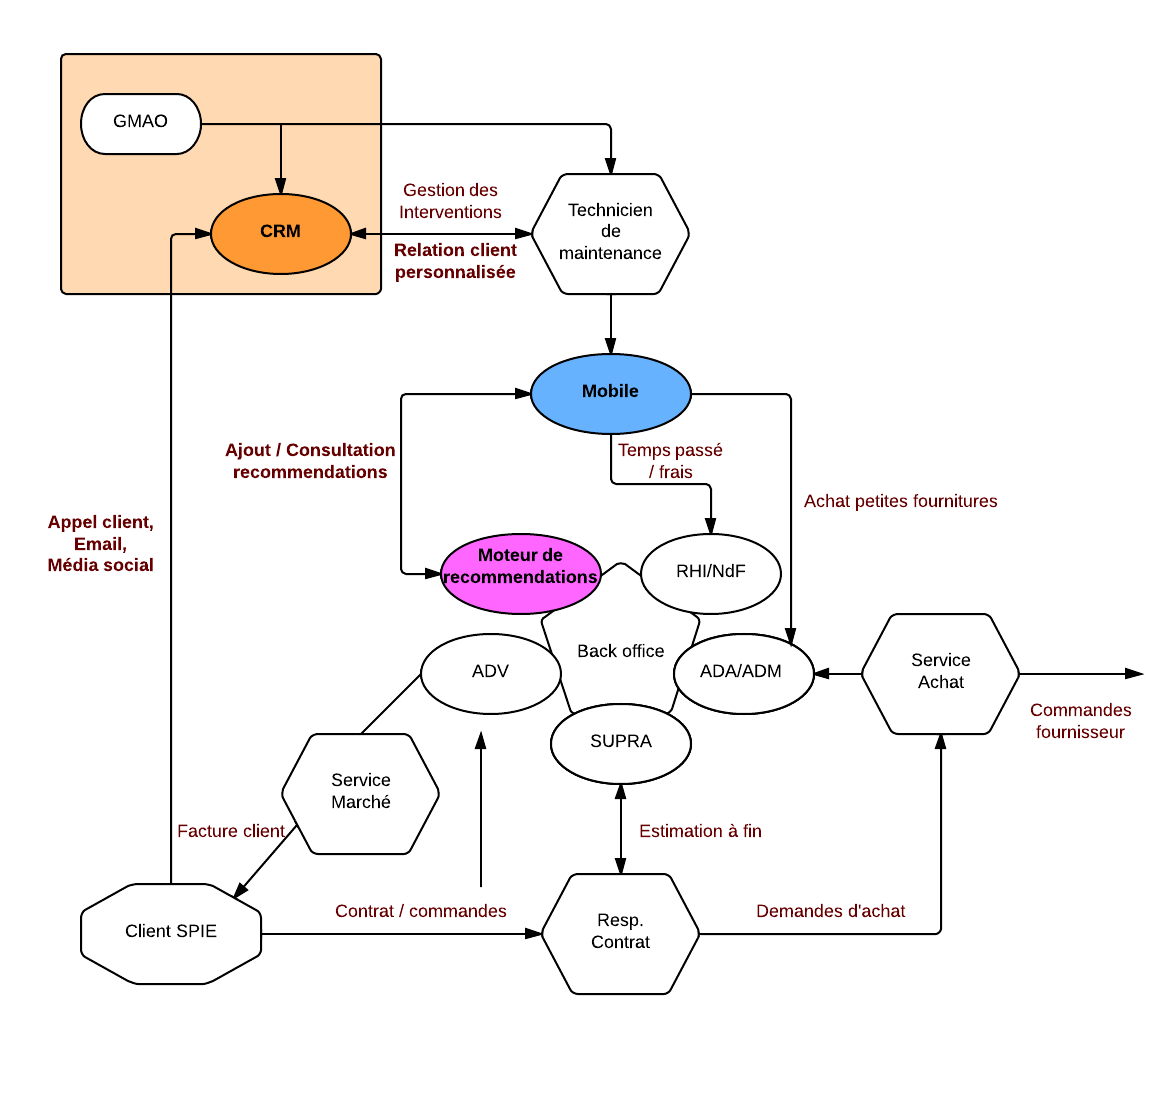
\includegraphics[width=1\linewidth]{images/cartographie_applicative_amelioree.png}
	\caption{Nouvelle architecture applicative}
	\label{fig:nouvelleArchitectureApplicative}
\end{figure}

